% Options for packages loaded elsewhere
\PassOptionsToPackage{unicode}{hyperref}
\PassOptionsToPackage{hyphens}{url}
%
\documentclass[
  ignorenonframetext,
]{beamer}
\usepackage{pgfpages}
\setbeamertemplate{caption}[numbered]
\setbeamertemplate{caption label separator}{: }
\setbeamercolor{caption name}{fg=normal text.fg}
\beamertemplatenavigationsymbolsempty
% Prevent slide breaks in the middle of a paragraph
\widowpenalties 1 10000
\raggedbottom
\setbeamertemplate{part page}{
  \centering
  \begin{beamercolorbox}[sep=16pt,center]{part title}
    \usebeamerfont{part title}\insertpart\par
  \end{beamercolorbox}
}
\setbeamertemplate{section page}{
  \centering
  \begin{beamercolorbox}[sep=12pt,center]{part title}
    \usebeamerfont{section title}\insertsection\par
  \end{beamercolorbox}
}
\setbeamertemplate{subsection page}{
  \centering
  \begin{beamercolorbox}[sep=8pt,center]{part title}
    \usebeamerfont{subsection title}\insertsubsection\par
  \end{beamercolorbox}
}
\AtBeginPart{
  \frame{\partpage}
}
\AtBeginSection{
  \ifbibliography
  \else
    \frame{\sectionpage}
  \fi
}
\AtBeginSubsection{
  \frame{\subsectionpage}
}

\usepackage{amsmath,amssymb}
\usepackage{lmodern}
\usepackage{iftex}
\ifPDFTeX
  \usepackage[T1]{fontenc}
  \usepackage[utf8]{inputenc}
  \usepackage{textcomp} % provide euro and other symbols
\else % if luatex or xetex
  \usepackage{unicode-math}
  \defaultfontfeatures{Scale=MatchLowercase}
  \defaultfontfeatures[\rmfamily]{Ligatures=TeX,Scale=1}
\fi
% Use upquote if available, for straight quotes in verbatim environments
\IfFileExists{upquote.sty}{\usepackage{upquote}}{}
\IfFileExists{microtype.sty}{% use microtype if available
  \usepackage[]{microtype}
  \UseMicrotypeSet[protrusion]{basicmath} % disable protrusion for tt fonts
}{}
\makeatletter
\@ifundefined{KOMAClassName}{% if non-KOMA class
  \IfFileExists{parskip.sty}{%
    \usepackage{parskip}
  }{% else
    \setlength{\parindent}{0pt}
    \setlength{\parskip}{6pt plus 2pt minus 1pt}}
}{% if KOMA class
  \KOMAoptions{parskip=half}}
\makeatother
\usepackage{xcolor}
\newif\ifbibliography
\setlength{\emergencystretch}{3em} % prevent overfull lines
\setcounter{secnumdepth}{-\maxdimen} % remove section numbering


\providecommand{\tightlist}{%
  \setlength{\itemsep}{0pt}\setlength{\parskip}{0pt}}\usepackage{longtable,booktabs,array}
\usepackage{calc} % for calculating minipage widths
\usepackage{caption}
% Make caption package work with longtable
\makeatletter
\def\fnum@table{\tablename~\thetable}
\makeatother
\usepackage{graphicx}
\makeatletter
\def\maxwidth{\ifdim\Gin@nat@width>\linewidth\linewidth\else\Gin@nat@width\fi}
\def\maxheight{\ifdim\Gin@nat@height>\textheight\textheight\else\Gin@nat@height\fi}
\makeatother
% Scale images if necessary, so that they will not overflow the page
% margins by default, and it is still possible to overwrite the defaults
% using explicit options in \includegraphics[width, height, ...]{}
\setkeys{Gin}{width=\maxwidth,height=\maxheight,keepaspectratio}
% Set default figure placement to htbp
\makeatletter
\def\fps@figure{htbp}
\makeatother

\makeatletter
\makeatother
\makeatletter
\makeatother
\makeatletter
\@ifpackageloaded{caption}{}{\usepackage{caption}}
\AtBeginDocument{%
\ifdefined\contentsname
  \renewcommand*\contentsname{Table of contents}
\else
  \newcommand\contentsname{Table of contents}
\fi
\ifdefined\listfigurename
  \renewcommand*\listfigurename{List of Figures}
\else
  \newcommand\listfigurename{List of Figures}
\fi
\ifdefined\listtablename
  \renewcommand*\listtablename{List of Tables}
\else
  \newcommand\listtablename{List of Tables}
\fi
\ifdefined\figurename
  \renewcommand*\figurename{Figure}
\else
  \newcommand\figurename{Figure}
\fi
\ifdefined\tablename
  \renewcommand*\tablename{Table}
\else
  \newcommand\tablename{Table}
\fi
}
\@ifpackageloaded{float}{}{\usepackage{float}}
\floatstyle{ruled}
\@ifundefined{c@chapter}{\newfloat{codelisting}{h}{lop}}{\newfloat{codelisting}{h}{lop}[chapter]}
\floatname{codelisting}{Listing}
\newcommand*\listoflistings{\listof{codelisting}{List of Listings}}
\makeatother
\makeatletter
\@ifpackageloaded{caption}{}{\usepackage{caption}}
\@ifpackageloaded{subcaption}{}{\usepackage{subcaption}}
\makeatother
\makeatletter
\@ifpackageloaded{tcolorbox}{}{\usepackage[many]{tcolorbox}}
\makeatother
\makeatletter
\@ifundefined{shadecolor}{\definecolor{shadecolor}{rgb}{.97, .97, .97}}
\makeatother
\makeatletter
\makeatother
\ifLuaTeX
  \usepackage{selnolig}  % disable illegal ligatures
\fi
\IfFileExists{bookmark.sty}{\usepackage{bookmark}}{\usepackage{hyperref}}
\IfFileExists{xurl.sty}{\usepackage{xurl}}{} % add URL line breaks if available
\urlstyle{same} % disable monospaced font for URLs
\hypersetup{
  pdftitle={Annotation goes distributional:},
  pdfauthor={Chiara Paolini},
  hidelinks,
  pdfcreator={LaTeX via pandoc}}

\title{Annotation goes distributional:}
\subtitle{Modeling semantic predictors of the dative alternation using
vector space models}
\author{Chiara Paolini}
\date{}

\begin{document}
\frame{\titlepage}
\ifdefined\Shaded\renewenvironment{Shaded}{\begin{tcolorbox}[sharp corners, enhanced, frame hidden, boxrule=0pt, interior hidden, borderline west={3pt}{0pt}{shadecolor}, breakable]}{\end{tcolorbox}}\fi

\begin{frame}{Outline}
\protect\hypertarget{outline}{}
\begin{itemize}
\tightlist
\item
  Introduction: the dative alternation
\item
  From vectors to predictors
\item
  Forests and clouds
\item
  Insights and further research
\end{itemize}

\note{In this talk, I would like to introduce you to the first case
study of my PhD research project called ``How much does meaning matter?
A fresh look at grammatical alternations''. The goal of this research is
to examine if and how the way people choose between different ways of
saying the same thing (i.e., grammatical alternations) depends on the
meaning of the words in the utterance. I will start by introduce you to
the dative alternation, our case study, and how lexical semantics is
traditionally modeled in variationist linguistics. Then, I will
illustrate our proposal, namely automatically-generated semantic
predictors using DS techniques, and finally I will discuss the analyses
and the results obtained from our first case study using type-level
distributional semantic predictors.}
\end{frame}

\hypertarget{introduction-the-dative-alternation}{%
\section{Introduction: the dative
alternation}\label{introduction-the-dative-alternation}}

\begin{frame}{The dative alternation}
\protect\hypertarget{the-dative-alternation}{}
\begin{enumerate}
\tightlist
\item
  \textbf{a) Ditransitive} dative variant
\end{enumerate}

{[}\emph{The waiter}{]}\textsubscript{subject}
{[}\emph{gave}{]}\textsubscript{verb} {[}\emph{my
cousin}{]}\textsubscript{recipient} {[}\emph{some
pizza}{]}\textsubscript{theme}

\begin{enumerate}
\tightlist
\item
  \textbf{b) Prepositional} dative variant
\end{enumerate}

{[}\emph{The waiter}{]}\textsubscript{subject}
{[}\emph{gave}{]}\textsubscript{verb} {[}\emph{some
pizza}{]}\textsubscript{theme} {[}\emph{to my
cousin}{]}\textsubscript{recipient}

\note{Let's dive into our case study. The DA is one of the most
investigated cases of grammatical alternation - where we define a GA as
``two or more constructions, called variants, with a highly similar
meaning. An A represents choice point for the individual speaker''.

In English, there are two ways, two variants to encode the dative
relation: the ditransitive dative construction (recipient-theme order),
and the prepositional dative construction (theme-recipient order).}
\end{frame}

\begin{frame}{Modelling grammatical alternations}
\protect\hypertarget{modelling-grammatical-alternations}{}
In previous literature, focus on three kinds of predictors:

\begin{enumerate}
\item
  \textbf{Formal predictors:} e.g., \emph{structural complexity of
  constituents} (e.g., presence of heavy postmodification),
  \emph{pronominality}, and \emph{constituent length} (in words,
  syllables, or similar)
\item
  \textbf{Information status‐related predictors:} e.g., \emph{givenness}
\item
  \textbf{Semantic, coarse-grained, higher-level predictors:} e.g.,
  \emph{animacy} (i.e., annotate for a binary distinction between
  animate and inanimate recipients -- see Bresnan et al.~2007)
\end{enumerate}

\note{To explore the correlation of choices between the two variants are
both implemented language-internal predictors as well as
language-external predictors (such as sex, race/ethnicity, etc).
Regarding the internal predictors, the traditional variationist approach
is fairly good at manually annotating for formal predictors, such as in
(1) and (2) for the dative alternation, but when it comes to the third
point, namely the semantic predictors, the VA would annotate only for
few semantic factors such as animacy. This is because (next slide)}
\end{frame}

\begin{frame}{Role of semantic predictors in alternation predictions}
\protect\hypertarget{role-of-semantic-predictors-in-alternation-predictions}{}
\textbf{Annotating for semantics is labor‐intensive and challenging to
perform objectively.}

\begin{itemize}
\tightlist
\item
  \emph{What role do semantic characteristics play in the choice of one
  of the two variants? At the current state of the research, we know
  very little about them.}
\end{itemize}

\textbf{We assume broad semantic equivalence of dative variants, but we
are interested in extent to which semantics of materials in argument
slots predicts choice.}

\note{Annotating for semantics is labor‐intensive and time-consuming,
and it's challenging to perform objectively and systematically. So if we
ask ourselves: What role do semantic characteristics play in the choice
of one of the two variants? We do not have a clear answer because we are
missing those data. And this is the research gap we want to cover.

In particular, we are interested how much the semantic characteristics
of the lexical material in the slots of the dative variants predict the
choice.}
\end{frame}

\hypertarget{from-vectors-to-predictors}{%
\section{From vectors to predictors}\label{from-vectors-to-predictors}}

\begin{frame}{Automatically-generated semantic predictors}
\protect\hypertarget{automatically-generated-semantic-predictors}{}
\textbf{Our suggestion: automatically-generated, corpus-based semantic
predictors using distributional semantic models (DSMs).}

\begin{itemize}
\item
  New inputs from DMSs: \textbf{more data, less annotation}
\item
  Distributional semantics is an usage-based model of meaning, based on
  the assumption that items that occur in similar contexts in a given
  corpus will be semantically similar, while those that occur in
  different contexts will be semantically different.
\end{itemize}

\note{(after reading the slides) DSMs can help us understanding and
bring to the light the semantic characteristics of the lexical context
in which those variants are embedded. In a nutshell, DS is a usage-based
model of meaning, based on the assumption that items that occur in
similar contexts in a given corpus will be semantically similar, while
those that occur in different contexts will be semantically different.
To do that, we operationalize the differences in the distribution of two
(or more) items by extracting their co-occurrences from corpora: those
differences can tell us something about the semantic relatedness of
items.}
\end{frame}

\begin{frame}{Examples: recipient type-lemmas}
\protect\hypertarget{examples-recipient-type-lemmas}{}
\begin{enumerate}
\tightlist
\item
  \textbf{DAT-4100}
\end{enumerate}

\begin{itemize}
\tightlist
\item
  {[}\emph{if I}{]}\textsubscript{subject}
  {[}\emph{gave}{]}\textsubscript{verb}
  {[}\emph{it}{]}\textsubscript{theme} {[}\emph{to the
  government}{]}\textsubscript{recipient} they would just waste it.
\end{itemize}

\begin{enumerate}
\setcounter{enumi}{1}
\tightlist
\item
  \textbf{DAT-4067}
\end{enumerate}

\begin{itemize}
\tightlist
\item
  {[}\emph{The judge}{]}\textsubscript{subject} {[}\emph{will usually,
  uh, give}{]}\textsubscript{verb}
  {[}\emph{custody}{]}\textsubscript{theme} {[}\emph{to the
  mother}{]}\textsubscript{recipient} ninety-seven percent of the time.
\end{itemize}

\note{But, what does it mean annotating predictors with DS? What we are
going to distributionally model are the recipient and the theme of the
alternation. (read the examples).}
\end{frame}

\begin{frame}{Matrix of recipients}
\protect\hypertarget{matrix-of-recipients}{}
\begin{longtable}[]{@{}
  >{\raggedright\arraybackslash}p{(\columnwidth - 10\tabcolsep) * \real{0.1644}}
  >{\raggedright\arraybackslash}p{(\columnwidth - 10\tabcolsep) * \real{0.1644}}
  >{\raggedright\arraybackslash}p{(\columnwidth - 10\tabcolsep) * \real{0.1644}}
  >{\raggedright\arraybackslash}p{(\columnwidth - 10\tabcolsep) * \real{0.1644}}
  >{\raggedright\arraybackslash}p{(\columnwidth - 10\tabcolsep) * \real{0.1644}}
  >{\raggedright\arraybackslash}p{(\columnwidth - 10\tabcolsep) * \real{0.1644}}@{}}
\toprule()
\begin{minipage}[b]{\linewidth}\raggedright
\end{minipage} & \begin{minipage}[b]{\linewidth}\raggedright
daughter/nn
\end{minipage} & \begin{minipage}[b]{\linewidth}\raggedright
europe/np
\end{minipage} & \begin{minipage}[b]{\linewidth}\raggedright
it/pp
\end{minipage} & \begin{minipage}[b]{\linewidth}\raggedright
dad/nn
\end{minipage} & \begin{minipage}[b]{\linewidth}\raggedright
troop/nn
\end{minipage} \\
\midrule()
\endhead
\begin{minipage}[t]{\linewidth}\raggedright
\textbf{government/nn}
\end{minipage} & -1.23 & 3.23 & 0.21 & 0.0 & 2.59 \\
\begin{minipage}[t]{\linewidth}\raggedright
\textbf{mother/nn}
\end{minipage} & 4.36 & 0.0 & 1.65 & 2.89 & 0.0 \\
\begin{minipage}[t]{\linewidth}\raggedright
\textbf{advance/nn}
\end{minipage} & -2.32 & 2.09 & 0.0 & -0.59 & 3.67 \\
\bottomrule()
\end{longtable}

\begin{itemize}
\tightlist
\item
  \textbf{\emph{Dative alternation dataset from Szmrecsanyi et
  al.~(2017)}}, which covers \textbf{N = 1,190} dative observations in
  contemporary \textbf{spoken American English} (Switchboard corpus)
\item
  Corpus for building DMSs: \emph{\textbf{Corpus of Contemporary
  American English} (COCA),} spoken register (ca. \textbf{127 million}
  tokens)
\end{itemize}

\note{In this first part of the study, we implemented what we call a
\textbf{type-level model}.

Let's consider only the group of recipients, here exemplified by
government/nn and mother/nn.~As you can see in this co-occurence matrix,
each row represents a target-words from the recipient slot: the
aggregation of the frequencies between the TW and the CW constitutes a
\textbf{word-type vector}. What you see here are raw frequencies
transformed, or better, weighted using \textbf{association strength
measures, such as PPMI}, that allow the model to bring up to the light
the informative semantic relationships between the words.

Building a DS model, means that we train a DS mode, a type-level one in
this case, with different parameters and compare them to pick the best
one BASED ON CUSTOMARY CRITERIA.

(read about the data set)}
\end{frame}

\hypertarget{forests-and-clouds}{%
\section{Forests and clouds}\label{forests-and-clouds}}

\begin{frame}{Clouds of recipients}
\protect\hypertarget{clouds-of-recipients}{}
\begin{figure}

{\centering 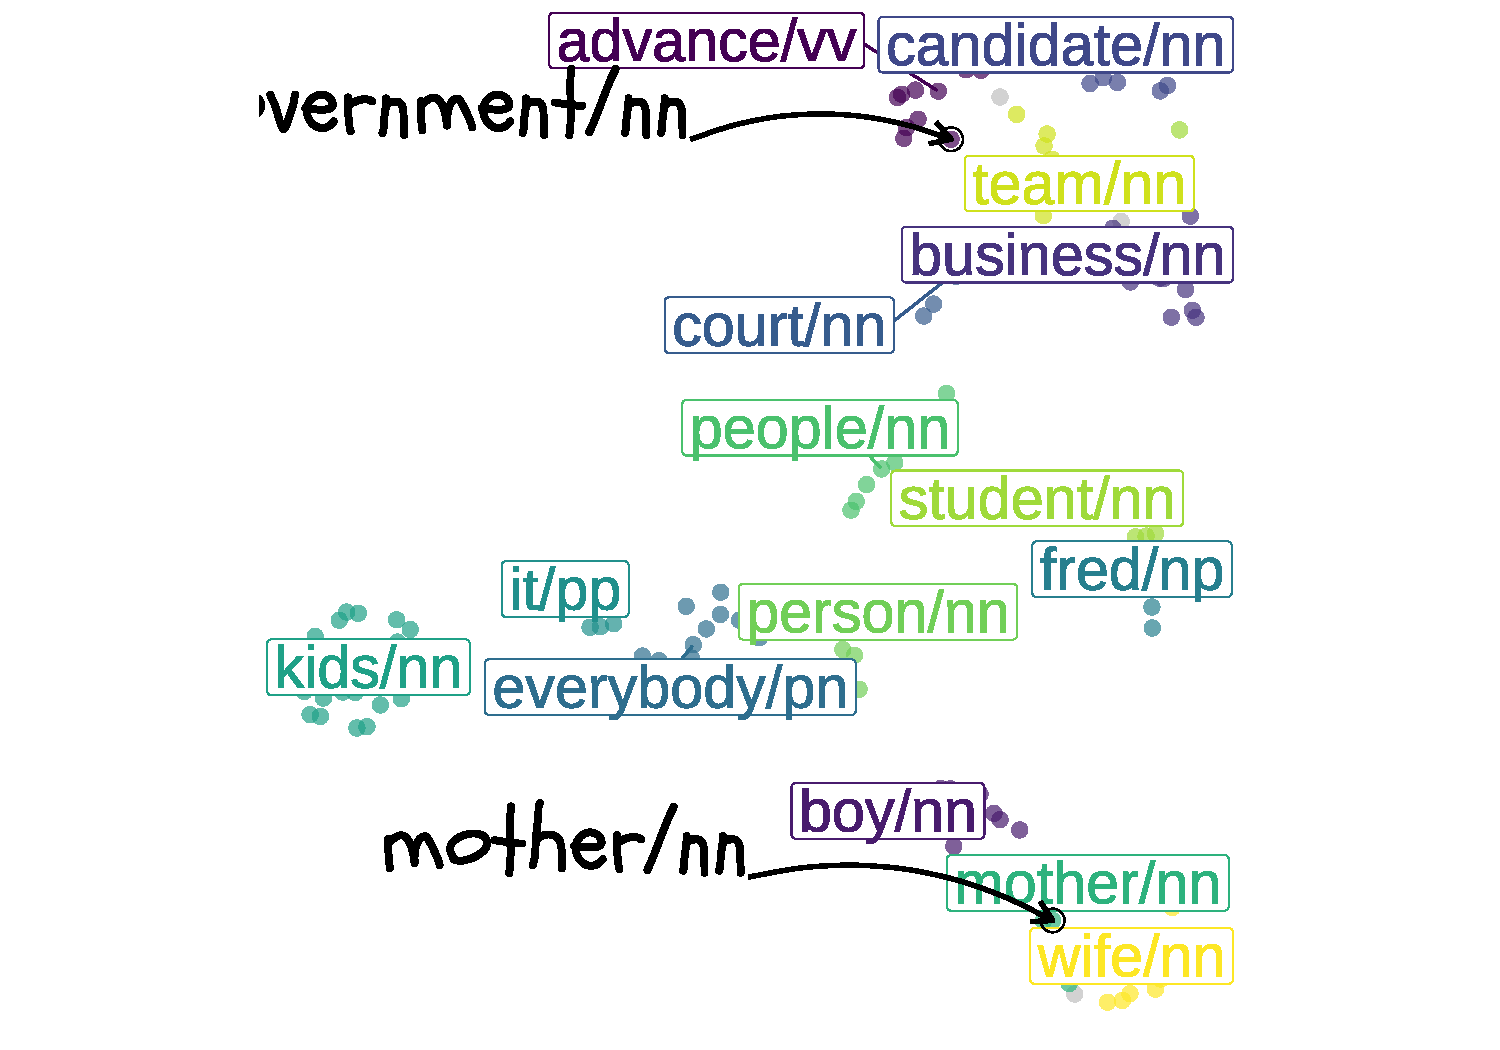
\includegraphics{index_files/figure-beamer/fig-tsne-r-1.pdf}

}

\caption{\label{fig-tsne-r}Scatterplot of recipient lemmas. Colors are
clusters, labelled by their central members.}

\end{figure}

\note{Building the semantic predictors using DS means identifying the
central member of the cluster (called medoid) from the data and grouping
the type-word vectors around them based on Euclidean distance metric. We
provide the number of clusters the algorithm should create: 3, 8, 15 in
our case.

Here, a nice plot of the clusters, or clouds as Mariana Montes says, of
the recipients in our best model. (The best model is
CS\_4\_ol\_10000\_ppmi\_10\_cosine\_k15 (with dimensionality
reduction)).

(describe the clusters)}
\end{frame}

\begin{frame}{Clouds of themes}
\protect\hypertarget{clouds-of-themes}{}
\begin{figure}

{\centering 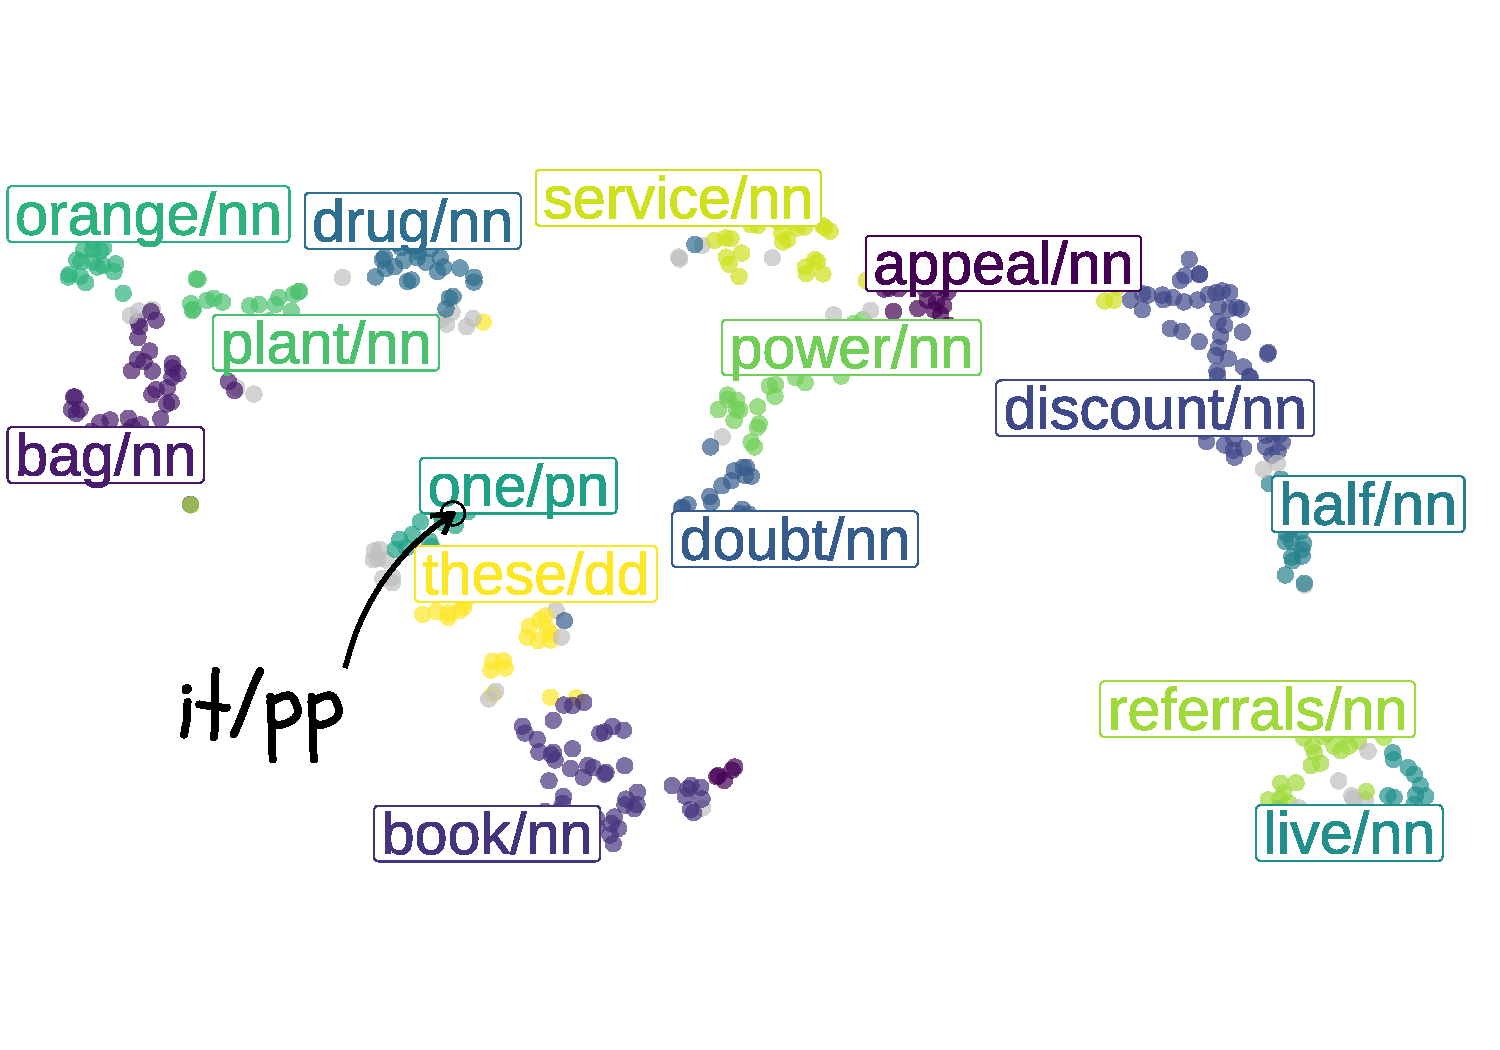
\includegraphics{index_files/figure-beamer/fig-tsne-t-1.pdf}

}

\caption{\label{fig-tsne-t}Scatterplot of themes lemmas. Colors are
clusters, labelled by their central members.}

\end{figure}
\end{frame}

\begin{frame}{From clouds to distributional semantic predictors}
\protect\hypertarget{from-clouds-to-distributional-semantic-predictors}{}
Each grouping of recipient/theme lemmas represents what we call
\textbf{\emph{distributional (semantic) predictor.}}

The prediction of the dative variants is based on the \textbf{membership
of the recipient/theme type-lemma in a particular semantic cluster.}

\note{To summarize, each grouping of recipient/theme lemmas represents
what we call \textbf{\emph{distributional (semantic) predictor.}} In
what follows, we predict dative choices based on the membership of the
recipients/themes in a particular semantic cluster by using two of the
most classic variationist statistical tools of analysis, Conditional
Random forest and Regression analysis.}
\end{frame}

\begin{frame}{Random forest}
\protect\hypertarget{random-forest}{}
\textbf{Random forest of traditional and distributional predictors}

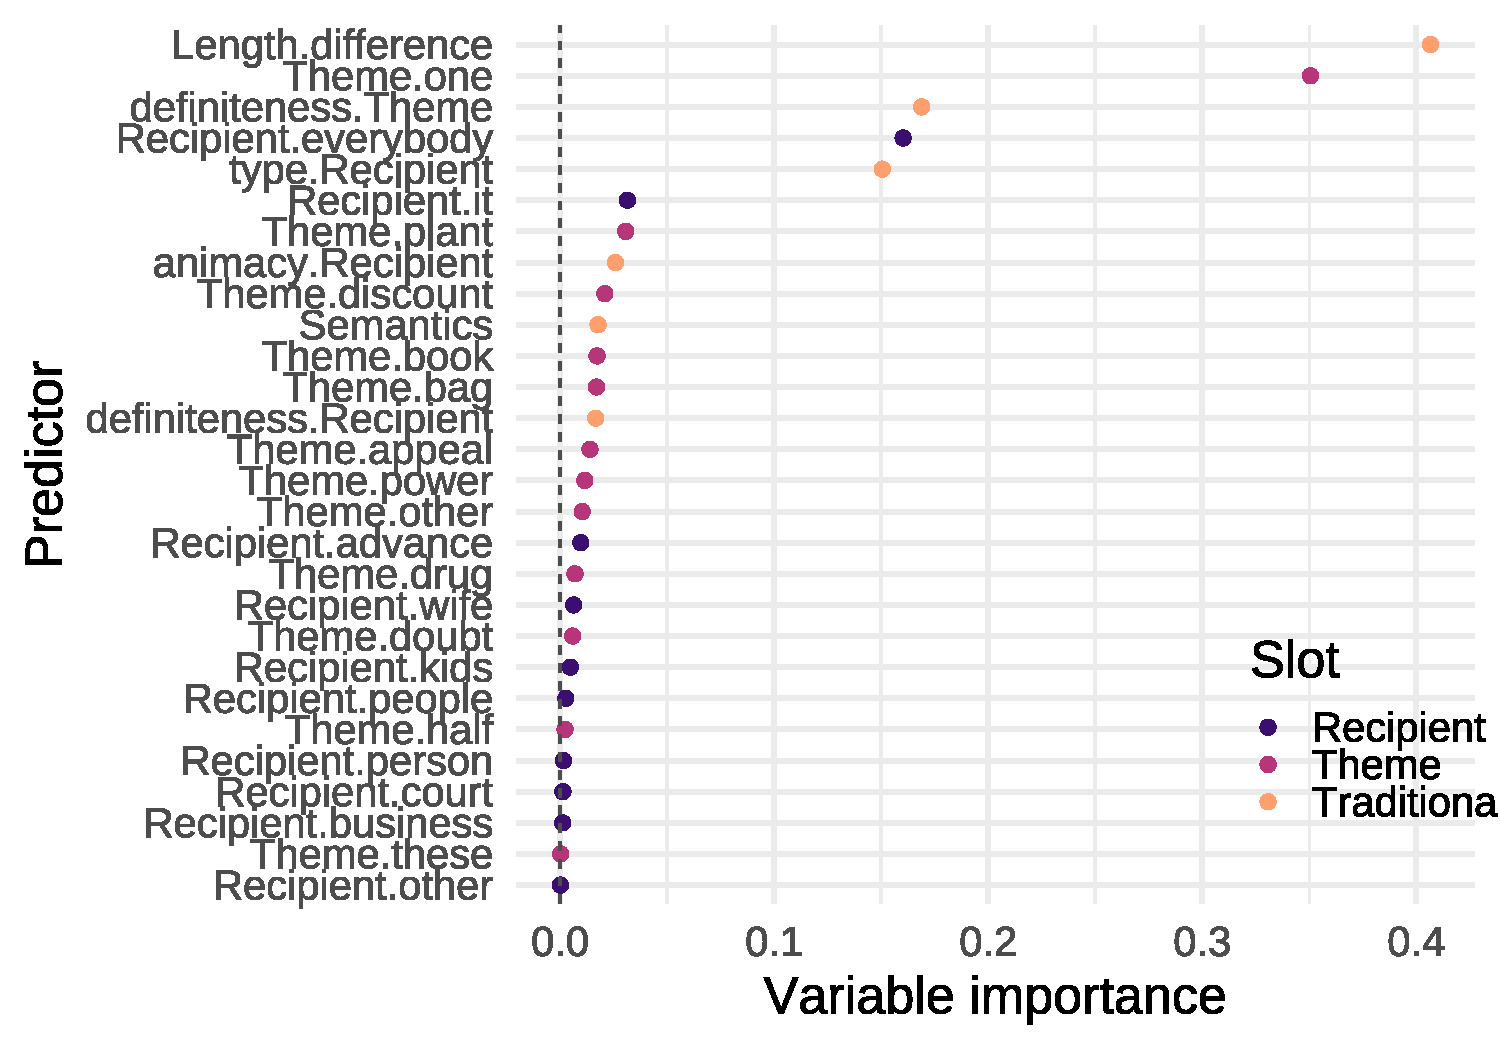
\includegraphics{index_files/figure-beamer/rf-full-1.pdf}

\note{CRF ia a recursive partitioning method based on conditional
inference trees: individual trees are `grown', and their predictions are
averaged. This statistical method can answer to the research question:
which linguistic factors help to predict the use of particular
linguistic variants? (explain the forest and show immediately the next
slide) - Do not insist too much on the pronominality}
\end{frame}

\begin{frame}{Inside the most important clouds}
\protect\hypertarget{inside-the-most-important-clouds}{}
\textbf{Theme.one:}

\begin{itemize}
\tightlist
\item
  \textbf{one/pn}, everything/pn, feel/nn, it/pp, lot/rr, one/nn,
  poke/nn, something/pn, stuff/nn, tempt/vv, that/dd, them/pp, thing/nn,
  try/nn, way/nn
\end{itemize}

\textbf{Recipient.everybody:}

\begin{itemize}
\tightlist
\item
  \textbf{everybody/pn}, anybody/pn, anyone/pn, anything/pn,
  everyone/pn, her/pp, him/pp, me/nn, me/pp, myself/pp, somebody/pn,
  stomach/nn, them/pp, us/pp, you/pp
\end{itemize}

\textbf{Recipient.it:}

\begin{itemize}
\tightlist
\item
  \textbf{it/pp}, that/dd, theory/nn, thing/nn
\end{itemize}
\end{frame}

\begin{frame}{Another look at the clouds: regression modelling}
\protect\hypertarget{another-look-at-the-clouds-regression-modelling}{}
\textbf{c-values of regression model with only traditional and
traditional+semantic predictors}

\textbf{Chi-square (Χ\textsuperscript{2}) goodness of fit (c-value)} =
non-parametric measure of how well a statistical model fits a set of
observations.

\begin{longtable}[]{@{}
  >{\raggedright\arraybackslash}p{(\columnwidth - 4\tabcolsep) * \real{0.4526}}
  >{\raggedright\arraybackslash}p{(\columnwidth - 4\tabcolsep) * \real{0.2737}}
  >{\raggedright\arraybackslash}p{(\columnwidth - 4\tabcolsep) * \real{0.2632}}@{}}
\toprule()
\begin{minipage}[b]{\linewidth}\raggedright
\end{minipage} & \begin{minipage}[b]{\linewidth}\raggedright
RM only trad predictors
\end{minipage} & \begin{minipage}[b]{\linewidth}\raggedright
RM trad+sem predictors
\end{minipage} \\
\midrule()
\endhead
\textbf{C-value for fixed effects} & 0.9844213 & 0.9747162 \\
\textbf{C-value for fixed and random effects} & 0.9854791 & 0.993123 \\
\bottomrule()
\end{longtable}

\note{We also analyzed the distributional predictors using RM, adding
them to the traditional, manually annotated, predictors. We are going to
have a quick glance at the main results.

We computed the c-value (\textbf{Concordance index C: goodness of fit})
for the two models with fixed and random effects: even if the model with
T+S performs better with the mixed effects, the higher c-v of 0.98 by
the Tmodel suggests how the traditional p performs better alone, than in
combination with the semantic ones.}
\end{frame}

\hypertarget{insights-and-further-research}{%
\section{Insights and further
research}\label{insights-and-further-research}}

\begin{frame}{Take-home messages}
\protect\hypertarget{take-home-messages}{}
\emph{``You shall choose a variant by the company it keeps!''}

\emph{(semi-cit. Firth 1955)}

\begin{enumerate}
\item
  Overall, there are some \textbf{distributional semantics clusters}
  that are \textbf{very predictive} of the alternation
\item
  Statistical analyses show how \textbf{traditional predictors
  outperform distributional semantics predictors} in terms of model
  performances
\end{enumerate}

\note{\begin{enumerate}
\setcounter{enumi}{1}
\tightlist
\item
  based on the c-value
\end{enumerate}}
\end{frame}

\begin{frame}{Directions for future research}
\protect\hypertarget{directions-for-future-research}{}
\begin{itemize}
\tightlist
\item
  \textbf{Other alternations:}

  \begin{itemize}
  \item
    \emph{Clausal complementation alternation} in the history of English
  \item
    \emph{Progressive alternation} in Italian
  \end{itemize}
\item
  \textbf{Experiment with token-level modeling}

  \begin{itemize}
  \tightlist
  \item
    see Montes (2021)
  \end{itemize}
\end{itemize}

\note{Token-level: in-depth analysis of the correlation of the single
occurrences of the lemmas with the context}
\end{frame}

\begin{frame}{Thoughts? Comments? Suggestions?}
\protect\hypertarget{thoughts-comments-suggestions}{}
\begin{figure}

{\centering 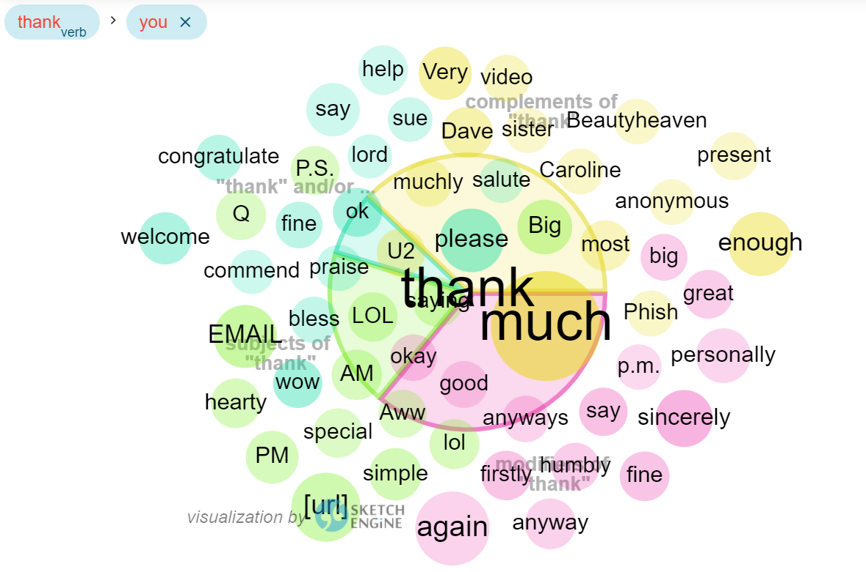
\includegraphics[width=7.05208in,height=\textheight]{images/thank_you.png}

}

\end{figure}

\textbf{\emph{chiara.paolini@kuleuven.be}}
\end{frame}

\begin{frame}{Traditional predictors}
\protect\hypertarget{traditional-predictors}{}
\begin{itemize}
\item
  \textbf{Recipient/Theme.type:} The annotation distinguishes between
  the following categories: (1) noun phrase; (2) personal pronoun; (3)
  demonstrative pronoun; (4) impersonal pronoun.
\item
  \textbf{Recipient/Theme.definiteness:} The annotation distinguishes
  between the following categories: (1) definite; (2) indefinite (3)
  definite proper noun.
\item
  \textbf{Recipient/Theme.animacy:} The annotation distinguishes between
  the following categories: (1) human and animal; (2) collective; (3)
  temporal; (4) locative; (5) inanimate.
\item
  \textbf{Length.difference:} The log difference between recipient and
  theme lengths (see Bresnan \& Ford 2010).
\item
  \textbf{Semantics (of dative verb):} (1) transfer; (2) communication;
  (3) abstract.
\item
  \textbf{Recipient/Theme.head:} Head lexeme of both the theme and the
  recipient.
\end{itemize}
\end{frame}

\begin{frame}{Inside the recipients clouds}
\protect\hypertarget{inside-the-recipients-clouds}{}
\begin{itemize}
\item
  \textbf{Recipient.advance}: advance/vv, america/np, arm/nn,
  country/nn, europe/np, government/nn, iranian/nn, nation/nn,
  nicaragua/np, russia/np, schwartzkopf/np, troop/nn, vietnamese/np
\item
  \textbf{Recipient.wife}: actress/nn, wife/nn, artist/nn, boss/nn,
  brother/nn, daughters/nn, friend/nn, husband/nn, kitty/np, ryan/np,
  sister/nn, thomases/np, trek/np
\item
  Recipient.kids: agencies/nn

  2

  0.3443036000

  kids/nn

  16

  boys/nn

  2

  0.5979984000

  kids/nn

  20

  businesses/nn

  2

  0.4080819000

  kids/nn

  29

  companies/nn

  2

  0.5218712000

  kids/nn

  33

  countries/nn

  2

  0.5652321000

  kids/nn

  37

  criminals/nn

  2

  0.3794335700

  kids/nn

  42

  dogs/nn

  2

  0.5007423000

  kids/nn

  43

  employees/nn

  2

  0.4876230700

  kids/nn

  56

  friends/nn

  2

  0.4518532500

  kids/nn

  60

  grandparents/nn

  2

  0.3280267400

  kids/nn

  66

  guys/nn

  2

  0.3701141800

  kids/nn

  70

  horses/nn

  2

  0.3475765000

  kids/nn

  72

  houses/nn

  2

  0.5975894300

  kids/nn

  82

  kids/nn

  2

  0.6238054000

  kids/nn

  95

  members/nn

  2

  0.4905860400

  kids/nn

  104

  parents/nn

  2

  0.5942958000

  kids/nn

  113

  rashad/np

  2

  0.3486836900

  kids/nn

  124

  sons/nn

  2

  0.5616968000

  kids/nn

  127

  students/nn

  2

  0.4786918000

  kids/nn

  135

  things/nn

  2

  0.4555949600

  kids/nn

  141

  twins/nn

  2

  0.5751200300

  kids/nn

  152

  women/nn
\end{itemize}
\end{frame}



\end{document}
